% Options for packages loaded elsewhere
\PassOptionsToPackage{unicode}{hyperref}
\PassOptionsToPackage{hyphens}{url}
%
\documentclass[
  ignorenonframetext,
  aspectratio=169,
]{beamer}
\usepackage{pgfpages}
\setbeamertemplate{caption}[numbered]
\setbeamertemplate{caption label separator}{: }
\setbeamercolor{caption name}{fg=normal text.fg}
\beamertemplatenavigationsymbolsempty
% Prevent slide breaks in the middle of a paragraph
\widowpenalties 1 10000
\raggedbottom
\setbeamertemplate{part page}{
  \centering
  \begin{beamercolorbox}[sep=16pt,center]{part title}
    \usebeamerfont{part title}\insertpart\par
  \end{beamercolorbox}
}
\setbeamertemplate{section page}{
  \centering
  \begin{beamercolorbox}[sep=12pt,center]{part title}
    \usebeamerfont{section title}\insertsection\par
  \end{beamercolorbox}
}
\setbeamertemplate{subsection page}{
  \centering
  \begin{beamercolorbox}[sep=8pt,center]{part title}
    \usebeamerfont{subsection title}\insertsubsection\par
  \end{beamercolorbox}
}
\AtBeginPart{
  \frame{\partpage}
}
\AtBeginSection{
  \ifbibliography
  \else
    \frame{\sectionpage}
  \fi
}
\AtBeginSubsection{
  \frame{\subsectionpage}
}

\usepackage{amsmath,amssymb}
\usepackage{iftex}
\ifPDFTeX
  \usepackage[T1]{fontenc}
  \usepackage[utf8]{inputenc}
  \usepackage{textcomp} % provide euro and other symbols
\else % if luatex or xetex
  \usepackage{unicode-math}
  \defaultfontfeatures{Scale=MatchLowercase}
  \defaultfontfeatures[\rmfamily]{Ligatures=TeX,Scale=1}
\fi
\usepackage{lmodern}
\usetheme[]{default}
\ifPDFTeX\else  
    % xetex/luatex font selection
\fi
% Use upquote if available, for straight quotes in verbatim environments
\IfFileExists{upquote.sty}{\usepackage{upquote}}{}
\IfFileExists{microtype.sty}{% use microtype if available
  \usepackage[]{microtype}
  \UseMicrotypeSet[protrusion]{basicmath} % disable protrusion for tt fonts
}{}
\makeatletter
\@ifundefined{KOMAClassName}{% if non-KOMA class
  \IfFileExists{parskip.sty}{%
    \usepackage{parskip}
  }{% else
    \setlength{\parindent}{0pt}
    \setlength{\parskip}{6pt plus 2pt minus 1pt}}
}{% if KOMA class
  \KOMAoptions{parskip=half}}
\makeatother
\usepackage{xcolor}
\newif\ifbibliography
\setlength{\emergencystretch}{3em} % prevent overfull lines
\setcounter{secnumdepth}{-\maxdimen} % remove section numbering

\usepackage{color}
\usepackage{fancyvrb}
\newcommand{\VerbBar}{|}
\newcommand{\VERB}{\Verb[commandchars=\\\{\}]}
\DefineVerbatimEnvironment{Highlighting}{Verbatim}{commandchars=\\\{\}}
% Add ',fontsize=\small' for more characters per line
\usepackage{framed}
\definecolor{shadecolor}{RGB}{241,243,245}
\newenvironment{Shaded}{\begin{snugshade}}{\end{snugshade}}
\newcommand{\AlertTok}[1]{\textcolor[rgb]{0.68,0.00,0.00}{#1}}
\newcommand{\AnnotationTok}[1]{\textcolor[rgb]{0.37,0.37,0.37}{#1}}
\newcommand{\AttributeTok}[1]{\textcolor[rgb]{0.40,0.45,0.13}{#1}}
\newcommand{\BaseNTok}[1]{\textcolor[rgb]{0.68,0.00,0.00}{#1}}
\newcommand{\BuiltInTok}[1]{\textcolor[rgb]{0.00,0.23,0.31}{#1}}
\newcommand{\CharTok}[1]{\textcolor[rgb]{0.13,0.47,0.30}{#1}}
\newcommand{\CommentTok}[1]{\textcolor[rgb]{0.37,0.37,0.37}{#1}}
\newcommand{\CommentVarTok}[1]{\textcolor[rgb]{0.37,0.37,0.37}{\textit{#1}}}
\newcommand{\ConstantTok}[1]{\textcolor[rgb]{0.56,0.35,0.01}{#1}}
\newcommand{\ControlFlowTok}[1]{\textcolor[rgb]{0.00,0.23,0.31}{#1}}
\newcommand{\DataTypeTok}[1]{\textcolor[rgb]{0.68,0.00,0.00}{#1}}
\newcommand{\DecValTok}[1]{\textcolor[rgb]{0.68,0.00,0.00}{#1}}
\newcommand{\DocumentationTok}[1]{\textcolor[rgb]{0.37,0.37,0.37}{\textit{#1}}}
\newcommand{\ErrorTok}[1]{\textcolor[rgb]{0.68,0.00,0.00}{#1}}
\newcommand{\ExtensionTok}[1]{\textcolor[rgb]{0.00,0.23,0.31}{#1}}
\newcommand{\FloatTok}[1]{\textcolor[rgb]{0.68,0.00,0.00}{#1}}
\newcommand{\FunctionTok}[1]{\textcolor[rgb]{0.28,0.35,0.67}{#1}}
\newcommand{\ImportTok}[1]{\textcolor[rgb]{0.00,0.46,0.62}{#1}}
\newcommand{\InformationTok}[1]{\textcolor[rgb]{0.37,0.37,0.37}{#1}}
\newcommand{\KeywordTok}[1]{\textcolor[rgb]{0.00,0.23,0.31}{#1}}
\newcommand{\NormalTok}[1]{\textcolor[rgb]{0.00,0.23,0.31}{#1}}
\newcommand{\OperatorTok}[1]{\textcolor[rgb]{0.37,0.37,0.37}{#1}}
\newcommand{\OtherTok}[1]{\textcolor[rgb]{0.00,0.23,0.31}{#1}}
\newcommand{\PreprocessorTok}[1]{\textcolor[rgb]{0.68,0.00,0.00}{#1}}
\newcommand{\RegionMarkerTok}[1]{\textcolor[rgb]{0.00,0.23,0.31}{#1}}
\newcommand{\SpecialCharTok}[1]{\textcolor[rgb]{0.37,0.37,0.37}{#1}}
\newcommand{\SpecialStringTok}[1]{\textcolor[rgb]{0.13,0.47,0.30}{#1}}
\newcommand{\StringTok}[1]{\textcolor[rgb]{0.13,0.47,0.30}{#1}}
\newcommand{\VariableTok}[1]{\textcolor[rgb]{0.07,0.07,0.07}{#1}}
\newcommand{\VerbatimStringTok}[1]{\textcolor[rgb]{0.13,0.47,0.30}{#1}}
\newcommand{\WarningTok}[1]{\textcolor[rgb]{0.37,0.37,0.37}{\textit{#1}}}

\providecommand{\tightlist}{%
  \setlength{\itemsep}{0pt}\setlength{\parskip}{0pt}}\usepackage{longtable,booktabs,array}
\usepackage{calc} % for calculating minipage widths
\usepackage{caption}
% Make caption package work with longtable
\makeatletter
\def\fnum@table{\tablename~\thetable}
\makeatother
\usepackage{graphicx}
\makeatletter
\def\maxwidth{\ifdim\Gin@nat@width>\linewidth\linewidth\else\Gin@nat@width\fi}
\def\maxheight{\ifdim\Gin@nat@height>\textheight\textheight\else\Gin@nat@height\fi}
\makeatother
% Scale images if necessary, so that they will not overflow the page
% margins by default, and it is still possible to overwrite the defaults
% using explicit options in \includegraphics[width, height, ...]{}
\setkeys{Gin}{width=\maxwidth,height=\maxheight,keepaspectratio}
% Set default figure placement to htbp
\makeatletter
\def\fps@figure{htbp}
\makeatother

% ============================================================
% StatLab Beamer Theme — Custom Header
% Mirrors the color scheme and layout of custom.scss (RevealJS)
% ============================================================

% ── COLORS (matches custom.scss variables) ───────────────────
\usepackage{xcolor}
\usepackage{pifont}

\definecolor{statprimary}{HTML}{2c3e50}    % dark gray-blue (body text)
\definecolor{statsecondary}{HTML}{2980b9}  % blue (structure, links)
\definecolor{statyale}{HTML}{00356b}       % Yale blue (footer)

% Box backgrounds
% Two-color system: Yale blue + statsecondary blue dominate.
% Orange (#FF6600) reserved for key warnings / key findings only.
\definecolor{stataccbg}{HTML}{e8f4f8}      % light cyan bg  — default block body
\definecolor{statorange}{HTML}{FF6600}     % orange         — alert / key finding header
\definecolor{statorangebg}{HTML}{FFF2E6}   % pale orange bg — alert body
\definecolor{statexbg}{HTML}{e6eef5}       % pale Yale-blue bg — example / Sam block body
\definecolor{statproof}{HTML}{95a5a6}      % gray           — proof (rarely used)
\definecolor{statproofbg}{HTML}{f9f9f9}    % light gray bg

% ── FONT: CMU Serif (LaTeX default) ─────────────────────────
% Switch Beamer from its default sans-serif to the classic serif.
\usefonttheme{serif}
% For XeLaTeX, explicitly select the OpenType CMU Serif face:
\setmainfont{CMU Serif}

% ── BEAMER COLORS ────────────────────────────────────────────

% Frame chrome
\setbeamercolor{frametitle}{bg=statprimary, fg=white}
\setbeamercolor{title}{fg=statprimary}
\setbeamercolor{subtitle}{fg=statsecondary}
\setbeamercolor{author}{fg=statprimary!70}
\setbeamercolor{date}{fg=statprimary!70}
\setbeamercolor{normal text}{fg=statprimary, bg=white}
\setbeamercolor{structure}{fg=statsecondary}

% Bullets and lists
\setbeamercolor{item}{fg=statsecondary}
\setbeamercolor{subitem}{fg=statsecondary!70}
\setbeamercolor{enumerate item}{fg=statsecondary}
\setbeamercolor{enumerate subitem}{fg=statsecondary!70}

% Bullet shape: filled circle (level 1), open circle (level 2), dash (level 3)
\setbeamertemplate{itemize item}{\small$\bullet$}
\setbeamertemplate{itemize subitem}{\small$\circ$}
\setbeamertemplate{itemize subsubitem}{\small\textendash}

% Default block — blue, mirrors .theorem / .lemma / .corollary
\setbeamercolor{block title}{fg=white, bg=statsecondary}
\setbeamercolor{block body}{bg=stataccbg, fg=statprimary}

% Alert block — orange (#FF6600), reserved for key warnings / findings
\setbeamercolor{block title alerted}{fg=white, bg=statorange}
\setbeamercolor{block body alerted}{bg=statorangebg, fg=statprimary}

% Example block — Yale blue, used for Sam callbacks and contextual examples
\setbeamercolor{block title example}{fg=white, bg=statyale}
\setbeamercolor{block body example}{bg=statexbg, fg=statprimary}

% ── FONT SIZES ───────────────────────────────────────────────
\setbeamerfont{title}{size=\LARGE, series=\bfseries}
\setbeamerfont{subtitle}{size=\large}
\setbeamerfont{frametitle}{size=\large, series=\bfseries}
\setbeamerfont{block title}{size=\normalsize, series=\bfseries}
\setbeamerfont{footline}{size=\scriptsize}

% ── FRAME TITLE ──────────────────────────────────────────────
\setbeamertemplate{navigation symbols}{}

\setbeamertemplate{frametitle}{%
  \nointerlineskip%
  \begin{beamercolorbox}[%
    wd=\paperwidth, ht=2.6ex, dp=0.9ex, leftskip=0.9em%
  ]{frametitle}%
    \usebeamerfont{frametitle}\insertframetitle%
  \end{beamercolorbox}%
}

% ── HEADLINE: presentation title, top-right (hidden on title slide) ──
\setbeamercolor{headline}{fg=statprimary!55, bg=white}
\setbeamertemplate{headline}{%
  \ifnum\insertframenumber>1%
    \begin{beamercolorbox}[wd=\paperwidth, ht=2.2ex, dp=0.5ex]{headline}%
      \hfill%
      \usebeamercolor[fg]{headline}{\fontsize{6.5}{8}\selectfont\inserttitle}%
      \hspace*{0.9em}%
    \end{beamercolorbox}%
  \else%
    \vspace{2.7ex}% reserve same height on title slide so frame title aligns
  \fi%
}

% ── FOOTER: branding + slide number (no logo) ────────────────
\setbeamertemplate{footline}{%
  {\color{statprimary!25}\hrule height 0.4pt}%
  \begin{beamercolorbox}[wd=\paperwidth, ht=2.4ex, dp=1.4ex]{footline}%
    \hspace*{0.9em}%
    \textcolor{statyale}{\fontfamily{qpl}\selectfont Yale Library $|$ StatLab}%
    \hfill%
    \textcolor{statprimary!50}{\insertframenumber\,/\,\inserttotalframenumber}%
    \hspace*{0.9em}%
  \end{beamercolorbox}%
}

% ── IMAGE CONSTRAINTS ────────────────────────────────────────
% Keep images within the content area so they never bleed into the footer.
% max-width = full text column; max-height = 65 % of the frame text height.
\usepackage{graphicx}
\setkeys{Gin}{width=\linewidth, height=0.65\textheight, keepaspectratio}

% ── TITLE PAGE ───────────────────────────────────────────────
\setbeamertemplate{title page}{%
  \vspace*{2.5em}%
  \begin{beamercolorbox}[sep=0pt, left]{title}%
    \usebeamerfont{title}\usebeamercolor[fg]{title}\inserttitle\par%
  \end{beamercolorbox}%
  \vspace*{0.5em}%
  \begin{beamercolorbox}[sep=0pt, left]{subtitle}%
    \usebeamerfont{subtitle}\usebeamercolor[fg]{subtitle}\insertsubtitle\par%
  \end{beamercolorbox}%
  \vspace*{1.8em}%
  \begin{beamercolorbox}[sep=0pt, left]{author}%
    \usebeamerfont{author}\usebeamercolor[fg]{author}\insertauthor\par%
  \end{beamercolorbox}%
  \vspace*{0.4em}%
  \begin{beamercolorbox}[sep=0pt, left]{date}%
    \usebeamerfont{date}\usebeamercolor[fg]{date}\insertdate\par%
  \end{beamercolorbox}%
}

% ── CUSTOM ENVIRONMENTS ──────────────────────────────────────
% Use these inside raw LaTeX blocks (```{=latex}) in your .qmd.
% Each mirrors the matching CSS class from the RevealJS theme.

% Definition — Yale blue (consistent with two-color palette)
\newenvironment{definitionblock}[1][Definition]{%
  \begingroup%
  \setbeamercolor{block title}{fg=white, bg=statyale}%
  \setbeamercolor{block body}{bg=statexbg, fg=statprimary}%
  \begin{block}{#1}%
}{%
  \end{block}%
  \endgroup%
}

% Lemma — blue, mirrors .lemma (same as default block)
\newenvironment{lemmablock}[1][Lemma]{%
  \begingroup%
  \begin{block}{#1}%
}{%
  \end{block}%
  \endgroup%
}

% Corollary — blue, mirrors .corollary (same as default block)
\newenvironment{corollaryblock}[1][Corollary]{%
  \begingroup%
  \begin{block}{#1}%
}{%
  \end{block}%
  \endgroup%
}

% Proof with QED square — gray, mirrors .proof
\newenvironment{proofblock}[1][Proof]{%
  \begingroup%
  \setbeamercolor{block title}{fg=white, bg=statproof}%
  \setbeamercolor{block body}{bg=statproofbg, fg=statprimary}%
  \begin{block}{\textit{#1}}%
  \itshape%
}{%
  \hfill$\square$%
  \end{block}%
  \endgroup%
}

% ── Workshop slide packages ───────────────────────────────────────────────
\usepackage{listings}
\usepackage{forest}
\usepackage{tikz}
\usetikzlibrary{arrows,arrows.meta,positioning,shapes.geometric,calc}
\usepackage{booktabs}
\usepackage{multicol}
\usepackage{array}
\usepackage{colortbl}   % \cellcolor / \rowcolor for highlighting table lookups

% ── Workshop color definitions ────────────────────────────────────────────
% Inline semantic colors (used in tables/code for before/after comparisons)
\definecolor{errorred}{RGB}{180,30,30}       % red  — bad examples, error states
\definecolor{highlightgreen}{RGB}{0,130,80}  % green — good examples, cached targets
\definecolor{commentgray}{RGB}{120,120,120}  % gray — code comments
\definecolor{warnorange}{RGB}{200,100,0}     % warm orange — string literals in code
\definecolor{lightblue}{RGB}{220,235,255}    % light blue — tikz fill

% ── Listings: tiny font, StatLab color accents ────────────────────────────
\lstset{
  basicstyle=\ttfamily\tiny,
  breaklines=true,
  frame=single,
  framerule=0.4pt,
  framesep=3pt,
  xleftmargin=8pt,
  xrightmargin=4pt,
  showstringspaces=false,
  commentstyle=\color{commentgray}\itshape,
  keywordstyle=\color{statsecondary}\bfseries,
  stringstyle=\color{warnorange},
  numbers=left,
  numberstyle=\tiny\color{gray!60},
  numbersep=5pt,
  tabsize=2,
  aboveskip=3pt,
  belowskip=3pt,
}

% ── Forest dirtree style ──────────────────────────────────────────────────
\forestset{
  dirtree/.style={
    for tree={
      font=\ttfamily\scriptsize,
      grow'=0,
      child anchor=west,
      parent anchor=south,
      anchor=west,
      calign=first,
      inner sep=1pt,
      outer sep=0pt,
      edge path={
        \noexpand\path [draw, \forestoption{edge}]
        (!u.south west) +(7.5pt,0) |- (.child anchor)
        \forestoption{edge label};
      },
      before typesetting nodes={
        if n=1{insert before={[,phantom]}}{}
      },
      fit=band,
      before computing xy={l=15pt},
    },
  }
}

% ── Quarto code block font size override ──────────────────────────────────
% Load fancyvrb explicitly so \DefineVerbatimEnvironment is always available,
% whether or not pandoc includes code blocks that trigger its auto-load.
\usepackage{fancyvrb}
\AtBeginDocument{%
  % Source code (syntax-highlighted input)
  \DefineVerbatimEnvironment{Highlighting}{Verbatim}{%
    commandchars=\\\{\},%
    fontsize=\small%
  }%
  % Printed results (plain verbatim) — matched to the input so a chunk
  % and its output read at one consistent size.
  \RecustomVerbatimEnvironment{verbatim}{Verbatim}{fontsize=\small}%
}

% ── Two-column shorthand colors for code comparisons ─────────────────────
\newcommand{\badlabel}{{\color{errorred}\textbf{$\boldsymbol{\times}$ Before}}}
\newcommand{\goodlabel}{{\color{highlightgreen}\textbf{\ding{51}~After}}}

% ── ORR Workshop rebuild macros (2025) ────────────────────────────────────

% Yale blue alias (for \color{yale})
\colorlet{yale}{statyale}

% Figure placeholder — reserves whitespace and flags human action needed
\newcommand{\figplaceholder}[1]{%
  \begin{center}%
  \fbox{\begin{minipage}{0.82\textwidth}%
  \centering\vspace{1.4cm}%
  {\large\color{gray} [FIGURE: #1]}\\[0.3cm]%
  {\small\color{gray}\itshape See [HUMAN INSTRUCTION] comment in source}%
  \vspace{1.4cm}%
  \end{minipage}}%
  \end{center}%
}

% Key finding callout (red alert block)
\newcommand{\findingbox}[1]{%
  \begin{alertblock}{Key Finding}%
  #1%
  \end{alertblock}%
}

% Title-less callout — example-block coloring, no title bar.
% Use where a block would otherwise invent a second heading under the frame title.
\newenvironment{notebox}{%
  \begin{center}%
  \begin{minipage}{0.95\textwidth}%
  \begin{beamercolorbox}[wd=\textwidth, sep=6pt]{block body example}%
}{%
  \end{beamercolorbox}%
  \end{minipage}%
  \end{center}%
}

% Inline pain/solution markers
\newcommand{\pain}[1]{{\color{errorred}\textbf{Problem:}} #1}
\newcommand{\solutiontag}[1]{{\color{yale}\textbf{Solution:}} #1}

% Parker Lab scenario callback — green example block
\newcommand{\samcallback}[1]{%
  \begin{exampleblock}{Parker Lab --- Sam's Problem}%
  \small #1%
  \end{exampleblock}%
}

% ── Named lstlisting styles ────────────────────────────────────────────────
% Override the global \tiny with \scriptsize for readability on slides.

\lstdefinestyle{Rcode}{%
  language=R,%
  basicstyle=\ttfamily\scriptsize,%
  backgroundcolor=\color{gray!8},%
  frame=single,%
  breaklines=true,%
  breakatwhitespace=false,%
  showstringspaces=false,%
  numbers=none,%
}

\lstdefinestyle{bashcode}{%
  language=bash,%
  basicstyle=\ttfamily\scriptsize,%
  backgroundcolor=\color{gray!8},%
  frame=single,%
  breaklines=true,%
  numbers=none,%
}

\lstdefinestyle{Pythoncode}{%
  language=Python,%
  basicstyle=\ttfamily\scriptsize,%
  backgroundcolor=\color{gray!8},%
  frame=single,%
  breaklines=true,%
  numbers=none,%
}

\lstdefinestyle{jsoncode}{%
  language={},%
  basicstyle=\ttfamily\scriptsize,%
  backgroundcolor=\color{gray!8},%
  frame=single,%
  breaklines=true,%
  numbers=none,%
  morestring=[b]",%
  stringstyle=\color{warnorange},%
}

\lstdefinestyle{yamlcode}{%
  language={},%
  basicstyle=\ttfamily\scriptsize,%
  backgroundcolor=\color{gray!8},%
  frame=single,%
  breaklines=true,%
  numbers=none,%
  morecomment=[l]{\#},%
  commentstyle=\color{commentgray}\itshape,%
}

\lstdefinestyle{textcode}{%
  language={},%
  basicstyle=\ttfamily\scriptsize,%
  backgroundcolor=\color{gray!8},%
  frame=none,%
  breaklines=true,%
  numbers=none,%
}
\makeatletter
\@ifpackageloaded{caption}{}{\usepackage{caption}}
\AtBeginDocument{%
\ifdefined\contentsname
  \renewcommand*\contentsname{Table of contents}
\else
  \newcommand\contentsname{Table of contents}
\fi
\ifdefined\listfigurename
  \renewcommand*\listfigurename{List of Figures}
\else
  \newcommand\listfigurename{List of Figures}
\fi
\ifdefined\listtablename
  \renewcommand*\listtablename{List of Tables}
\else
  \newcommand\listtablename{List of Tables}
\fi
\ifdefined\figurename
  \renewcommand*\figurename{Figure}
\else
  \newcommand\figurename{Figure}
\fi
\ifdefined\tablename
  \renewcommand*\tablename{Table}
\else
  \newcommand\tablename{Table}
\fi
}
\@ifpackageloaded{float}{}{\usepackage{float}}
\floatstyle{ruled}
\@ifundefined{c@chapter}{\newfloat{codelisting}{h}{lop}}{\newfloat{codelisting}{h}{lop}[chapter]}
\floatname{codelisting}{Listing}
\newcommand*\listoflistings{\listof{codelisting}{List of Listings}}
\makeatother
\makeatletter
\makeatother
\makeatletter
\@ifpackageloaded{caption}{}{\usepackage{caption}}
\@ifpackageloaded{subcaption}{}{\usepackage{subcaption}}
\makeatother
\ifLuaTeX
  \usepackage{selnolig}  % disable illegal ligatures
\fi
\usepackage{bookmark}

\IfFileExists{xurl.sty}{\usepackage{xurl}}{} % add URL line breaks if available
\urlstyle{same} % disable monospaced font for URLs
\hypersetup{
  pdftitle={Statistical Power},
  pdfauthor={Cole Brookson, MSc},
  hidelinks,
  pdfcreator={LaTeX via pandoc}}

\title{Statistical Power}
\author{Cole Brookson, MSc}
\date{2026-10-14}

\begin{document}
\frame{\titlepage}

\begin{frame}{Free statistical consulting for Yale researchers!}
\phantomsection\label{free-statistical-consulting-for-yale-researchers}
\vspace{2.8em}

\begin{center}

\large
Study design $\cdot$ analysis $\cdot$ visualization $\cdot$ theory.

\vspace{1.4em}

\normalsize
Walk-ins, appointments, and workshops --- free for all Yale affiliates.

\vspace{2.8em}

\textcolor{statsecondary}{%
  \large\textbf{library.yale.edu/statlab}%
}

\end{center}
\end{frame}

\begin{frame}{Introduction}
\phantomsection\label{introduction}
\vspace{1.4em}

\begin{center}
\large A committee, a reviewer, an IRB, or a funder asks: \textbf{how many subjects do you need?}
\end{center}

\begin{figure}

\centering{

\includegraphics[width=\textwidth,height=0.5\textheight]{./images/power-meme.png}

}

\caption{\label{fig-meme}All problems are solved with more power.}

\end{figure}%
\end{frame}

\begin{frame}{Schedule}
\phantomsection\label{schedule}
\vspace{0.3em}
\end{frame}

\begin{frame}{Learning Objectives}
\phantomsection\label{learning-objectives}
\vspace{0.3em}

\small By the end of the session you should be able to:

\vspace{0.4em}

\begin{center}
\begin{enumerate}
  \item Describe the formal definition of statistical power, and relate it to other quantities of interest 
  \item Generalize the formal definition of statistical power to an agnostic view of the "False negative" problem
  \item Calculate power from a closed form in the classic hypothesis testing framing 
  \item Understand and design an agnostic power calculation to quantify effect size recovery in an arbitrary model
\end{enumerate}
\end{center}
\end{frame}

\begin{frame}{False Negatives and False Positives}
\phantomsection\label{false-negatives-and-false-positives}
\begin{columns}[T]
\begin{column}{0.6\textwidth}
\begin{itemize}
\item
  Most diagnostic statistics seek to identify two types of errors:

  \begin{itemize}
  \tightlist
  \item
    \emph{False Positive} (\(\alpha\), Type I) refer to the probability
    that you will claim an effect is \emph{present} when the
    \textbf{null hypothesis is true}.
  \item
    \emph{False Negatives} (\(\beta\), Type II) refer to the probability
    that you will claim an effect is \emph{absent} when the \textbf{null
    hypothesis is false}.
  \end{itemize}
\item
  Power is what is left over from a false negative error:
  \(\text{power} = 1 - \beta\).
\end{itemize}
\end{column}

\begin{column}{0.4\textwidth}
\begin{figure}

\centering{

\includegraphics[width=\textwidth,height=0.5\textheight]{./images/cohen.png}

}

\caption{\label{fig-cohen}Dr.~Jacob Cohen (1923-1998)}

\end{figure}%
\end{column}
\end{columns}

\begin{center}
Power is \textbf{the probability of rejecting the null hypothesis when it is in fact false and should be rejected.}
\end{center}
\end{frame}

\begin{frame}{What is Statistical Power?}
\phantomsection\label{what-is-statistical-power}
\begin{itemize}
\item
  Less formally: power is a study's ability to \emph{distinguish signal
  from noise.}

  \begin{itemize}
  \tightlist
  \item
    The \emph{signal} is the real effect.
  \item
    The \emph{noise} is everything else (e.g., sampling variability,
    measurement error, differences between units, etc.)
  \end{itemize}
\end{itemize}
\end{frame}

\begin{frame}{What Power Looks Like}
\phantomsection\label{what-power-looks-like}
\begin{figure}[H]

{\centering 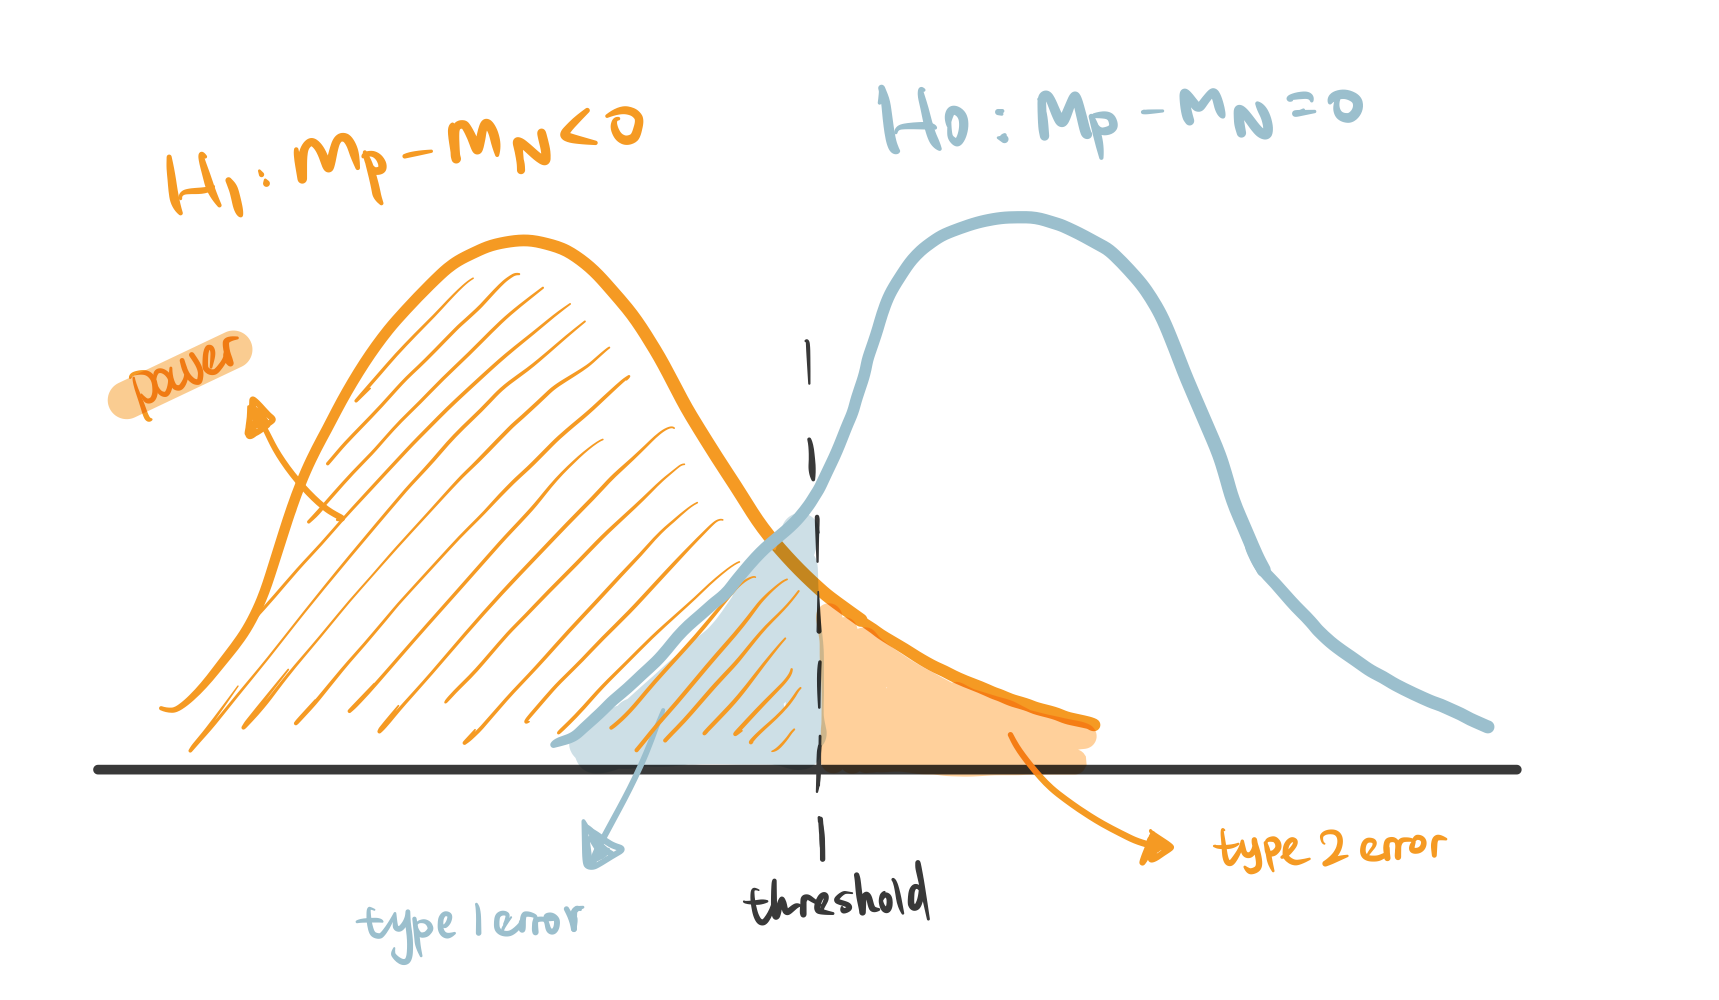
\includegraphics{../images/power-vis.png}

}

\caption{A nice illustration of the concept}

\end{figure}%
\end{frame}

\begin{frame}{Traditional Statistical Power \& Its Ingredients}
\phantomsection\label{traditional-statistical-power-its-ingredients}
\vskip0pt plus 1filll

When conducting power analysis, our goal is to derive the probability of
\emph{detecting} a positive effect when the null hypothesis is false.

\begin{itemize}
\tightlist
\item
  Many studies use \(\text{power} \geq 80\%\) (equivalently,
  \(\beta \leq 0.20\)) as a threshold:

  \begin{itemize}
  \tightlist
  \item
    Implies that there is a \(20\%\) chance that you will \emph{not}
    find an effect that is present
  \item
    Similar to \(\alpha=0.05\) being taken as natural law, uncritical
    choice of \(\beta\) should be discouraged
  \end{itemize}
\end{itemize}

\vskip0pt plus 1filll

\begin{center}
\textit{``surely, God loves the .06 nearly as much as the .05"} (Rosnow and Rosenthal, 1989)''
\end{center}
\end{frame}

\begin{frame}{Traditional Statistical Power \& Its Ingredients}
\phantomsection\label{traditional-statistical-power-its-ingredients-1}
\vskip0pt plus 1filll

So what do we need to actually calculate this? Well, the constituent
components to calculate \(1 - \beta\) are:

\begin{itemize}
\tightlist
\item
  \textbf{$\alpha$, the significance criterion}
\item
  \textbf{$N$, the sample size}
\item
  \textbf{$\delta$, the population effect size} \vskip0pt plus 1filll
\end{itemize}

\begin{center}
\textit{So,} you must be thinking, \textit{what's the formula?!}

\end{center}
\end{frame}

\begin{frame}{Traditional Statistical Power \& Its Ingredients}
\phantomsection\label{traditional-statistical-power-its-ingredients-2}
\vskip0pt plus 1filll

So what do we need to actually calculate this? Well, the constituent
components to calculate \(1 - \beta\) are:

\begin{itemize}
\tightlist
\item
  \textbf{$\alpha$, the significance criterion}
\item
  \textbf{$N$, the sample size}
\item
  \textbf{$\delta$, the population effect size} \vskip0pt plus 1filll
\end{itemize}

\begin{center}
\textit{So,} you must be thinking, \textit{what's the formula?!}

Well, as luck would have it, there isn't one. 
\end{center}
\end{frame}

\begin{frame}{Traditional Statistical Power \& Its Ingredients}
\phantomsection\label{traditional-statistical-power-its-ingredients-3}
\begin{center}
\Large
There isn't a formula for the calculation of power. There are many!
\end{center}
\end{frame}

\begin{frame}{Let's look at a case where we can find a closed form}
\phantomsection\label{lets-look-at-a-case-where-we-can-find-a-closed-form}
The formula depends entirely on what \emph{specific} test you want to
run. Here's an example. Let's make the following assumptions:

\begin{enumerate}
\tightlist
\item
  We have a completely randomized experiment, with two groups are
  selected to form a binary treatment, each group containing \(N \ 2\)
\item
  Assume the outcome variable is normally distributed, and the control
  group has mean \(\mu_c\) and the treatment group has \(\mu_t\)
\item
  The two groups have a shared standard deviation, \(\sigma\)
\end{enumerate}

We now say we want to perform a difference of means test, in the
two-tailed sense
\end{frame}

\begin{frame}{Let's look at a case where we can find a closed form}
\phantomsection\label{lets-look-at-a-case-where-we-can-find-a-closed-form-1}
Say we have the following hypothetical situation where we want to
compute power:

\begin{itemize}
\tightlist
\item
  A school is piloting a new \textbf{tutoring program}, and wants to
  know if it improves end-of-term test scores (out of 100)
\item
  Students are randomized into two groups, with one half getting
  tutoring
\item
  Untutored students average \(\mu_c = 72\)
\item
  The school will consider the program ``worth it'', if tutoring gets
  average scores to \(\mu_t = 75\)
\item
  Scores vary with \(\sigma = 10\)
\end{itemize}
\end{frame}

\begin{frame}{Let's look at a case where we can find a closed form}
\phantomsection\label{lets-look-at-a-case-where-we-can-find-a-closed-form-2}
The formula depends entirely on what \emph{specific} test you want to
run. Here's an example. Let's make the following assumptions:

\begin{enumerate}
\tightlist
\item
  We have a completely randomized experiment, with two groups are
  selected to form a binary treatment, each group containing \(N / 2\)
\item
  Assume the outcome variable is normally distributed, and the control
  group has mean \(\mu_c\) and the treatment group has \(\mu_t\)
\item
  The two groups have a shared standard deviation, \(\sigma\)
\end{enumerate}

We now say we want to perform a difference of means test, in the
two-tailed sense

\begin{center}
Luckily, in such a simple form, there's a nice asymptotic approximation for the power of the experiment
\end{center}
\end{frame}

\begin{frame}{Let's look at a case where we can find a closed form}
\phantomsection\label{lets-look-at-a-case-where-we-can-find-a-closed-form-3}
\[
1 - \beta = \Phi \left( \frac{ | \mu_t - \mu_c | \sqrt{N}}{2\sigma} - \Phi^{-1}\ \left(1-\frac{\alpha}{2}\right) \right)
\]

where \(\Phi\) is the cumulative distribution function of the standard
normal distribution, which is given by:

\[
\Phi(x) = \frac{1}{\sqrt{2\pi}} \int_{-\infty}^{x} e^{-u^2/2} \, du
\]

that is, the probability that a standard normal variable falls at or
below \(x\).
\end{frame}

\begin{frame}[fragile]{Let's look at a case where we can find a closed
form}
\phantomsection\label{lets-look-at-a-case-where-we-can-find-a-closed-form-4}
For the sake of completeness, we can, of course, do this in R:

\begin{Shaded}
\begin{Highlighting}[]
\NormalTok{two\_tailed\_power }\OtherTok{\textless{}{-}} \ControlFlowTok{function}\NormalTok{(mu\_t, mu\_c, std\_dev, alpha, n) \{}
\NormalTok{    effect\_in\_sd }\OtherTok{\textless{}{-}}\NormalTok{ (}\FunctionTok{abs}\NormalTok{(mu\_t }\SpecialCharTok{{-}}\NormalTok{ mu\_c) }\SpecialCharTok{*} \FunctionTok{sqrt}\NormalTok{(n)) }\SpecialCharTok{/}\NormalTok{ (}\DecValTok{2} \SpecialCharTok{*}\NormalTok{ std\_dev)}
\NormalTok{    critical\_val }\OtherTok{\textless{}{-}} \FunctionTok{qnorm}\NormalTok{(}\DecValTok{1} \SpecialCharTok{{-}}\NormalTok{ (alpha }\SpecialCharTok{/} \DecValTok{2}\NormalTok{)) }\CommentTok{\# phi \^{}\{{-}1\} is qnorm!}
\NormalTok{    power }\OtherTok{\textless{}{-}} \FunctionTok{pnorm}\NormalTok{(effect\_in\_sd }\SpecialCharTok{{-}}\NormalTok{ critical\_val)}
\NormalTok{    power}
\NormalTok{\}}

\FunctionTok{two\_tailed\_power}\NormalTok{(}\AttributeTok{mu\_t =} \DecValTok{75}\NormalTok{, }\AttributeTok{mu\_c =} \DecValTok{72}\NormalTok{, }\AttributeTok{std\_dev =} \DecValTok{10}\NormalTok{, }\AttributeTok{alpha =} \FloatTok{0.05}\NormalTok{, }\AttributeTok{n =} \DecValTok{400}\NormalTok{)}
\end{Highlighting}
\end{Shaded}

\begin{verbatim}
[1] 0.8508384
\end{verbatim}
\end{frame}

\begin{frame}{Let's look at a case where we can find a closed form}
\phantomsection\label{lets-look-at-a-case-where-we-can-find-a-closed-form-5}
But the standard use case, of course, is often to find a minimum sample
size that satisfies the requisite power.

\begin{itemize}
\tightlist
\item
  Without knowing our sample size, but knowing all the other points, how
  could we do this?
\item
  Do you have a guess for what the number for \(N\) is?
\end{itemize}
\end{frame}

\begin{frame}[fragile]{Let's look at a case where we can find a closed
form - sample size}
\phantomsection\label{lets-look-at-a-case-where-we-can-find-a-closed-form---sample-size}
Starting with our formula from before:

\[
1 - \beta = \Phi \left( \frac{ | \mu_t - \mu_c | \sqrt{N}}{2\sigma} - \Phi^{-1}\ \left(1-\frac{\alpha}{2}\right) \right)
\]

if we skip over some substitutions and simplification, we can get to:

\[
\boxed{N = \frac{4\sigma^2\,(z_{1-\alpha/2} + z_{1-\beta})^2}{(\mu_t - \mu_c)^2}}
\]

where our only two new values are the z-values for \(\alpha\) and
\(\beta\) respectively, which we know to be \(z_{1-\alpha/2} = 1.96\)
from memory or calculation, and \(z_{1-\beta}\) we can get via
\texttt{qnorm(0.8)} which ends up being \(\approx 0.84\).
\end{frame}

\begin{frame}{Let's look at a case where we can find a closed form -
sample size}
\phantomsection\label{lets-look-at-a-case-where-we-can-find-a-closed-form---sample-size-1}
\[
\boxed{N = \frac{4\sigma^2\,(z_{1-\alpha/2} + z_{1-\beta})^2}{(\mu_t - \mu_c)^2}}
\]

Your turn! See if you can adapt our function above using the equation
here that calculates a sample size that fulfills power = 0.8.
\end{frame}

\begin{frame}[fragile]{Let's look at a case where we can find a closed
form - sample size}
\phantomsection\label{lets-look-at-a-case-where-we-can-find-a-closed-form---sample-size-2}
So, using \[
\boxed{N = \frac{4\sigma^2\,(z_{1-\alpha/2} + z_{1-\beta})^2}{(\mu_t - \mu_c)^2}}
\]

we can write a function \emph{very} similar to our above function:

\begin{Shaded}
\begin{Highlighting}[]
\NormalTok{n\_required }\OtherTok{\textless{}{-}} \ControlFlowTok{function}\NormalTok{(mu\_t, mu\_c, std\_dev, alpha, power) \{}
\NormalTok{  z\_sum }\OtherTok{\textless{}{-}} \FunctionTok{qnorm}\NormalTok{(}\DecValTok{1} \SpecialCharTok{{-}}\NormalTok{ alpha }\SpecialCharTok{/} \DecValTok{2}\NormalTok{) }\SpecialCharTok{+} \FunctionTok{qnorm}\NormalTok{(power)}
  \DecValTok{4} \SpecialCharTok{*}\NormalTok{ std\_dev}\SpecialCharTok{\^{}}\DecValTok{2} \SpecialCharTok{*}\NormalTok{ z\_sum}\SpecialCharTok{\^{}}\DecValTok{2} \SpecialCharTok{/}\NormalTok{ (mu\_t }\SpecialCharTok{{-}}\NormalTok{ mu\_c)}\SpecialCharTok{\^{}}\DecValTok{2}
\NormalTok{\}}
\FunctionTok{n\_required}\NormalTok{(}\AttributeTok{mu\_t =} \DecValTok{75}\NormalTok{, }\AttributeTok{mu\_c =} \DecValTok{72}\NormalTok{, }\AttributeTok{std\_dev =} \DecValTok{10}\NormalTok{, }\AttributeTok{alpha =} \FloatTok{0.05}\NormalTok{, }\AttributeTok{power =} \FloatTok{0.80}\NormalTok{)}
\end{Highlighting}
\end{Shaded}

\begin{verbatim}
[1] 348.8391
\end{verbatim}

There's lots of ways to do this in mostly equivalent ways!
\end{frame}

\begin{frame}{But what about literally any other case?}
\phantomsection\label{but-what-about-literally-any-other-case}
There are lots of reasons why, even for simple problems, we don't want
to rely on such an approximation. For instance, what if you

\begin{enumerate}
\tightlist
\item
  don't assume a two-tailed test?
\item
  have clustering and want some sort of random effect?
\item
  are taking a Bayesian approach?
\item
  are using nonparametric statistics?
\end{enumerate}
\end{frame}

\begin{frame}{What should we do in those other cases?}
\phantomsection\label{what-should-we-do-in-those-other-cases}
\begin{itemize}
\tightlist
\item
  Even when power is not as clearly defined, there are still a whole
  range of things we still want to know about ``power''
\item
  Let's start relaxing our definition of power. We can, for now,
  consider it as:
\end{itemize}

\vskip50pt

\begin{center}
\textbf{The probability that we we \textcolor{red}{recover} a real effect, should one \textcolor{red}{exist}}
\end{center}
\end{frame}

\begin{frame}{What should we do in those other cases?}
\phantomsection\label{what-should-we-do-in-those-other-cases-1}
What would it mean then, to approach asking questions about power or
sample size in a more general sense where we may want to consider:

\vskip20pt

\begin{columns}[T]
\begin{column}{0.6\textwidth}
\begin{itemize}
\tightlist
\item
  Non-parametric approaches
\item
  Bayesian approaches
\item
  Or even just moderately more complicated study designs?
\end{itemize}

\vskip20pt

\begin{center}
\textbf{Well, we go gambling}
\end{center}
\end{column}

\begin{column}{0.4\textwidth}
\begin{figure}

\centering{

\includegraphics[width=\textwidth,height=0.5\textheight]{./images/casino.png}

}

\caption{\label{fig-casino}Oxford Casino Hotel}

\end{figure}%
\end{column}
\end{columns}
\end{frame}

\begin{frame}{An aside into the casinos at Monaco}
\phantomsection\label{an-aside-into-the-casinos-at-monaco}
\begin{columns}[T]
\begin{column}{0.6\textwidth}
\begin{itemize}
\tightlist
\item
  Monte Carlo refers to a broad class of methods wherein you use
  repeated random sampling to obtain some form of numerical result
\item
  It will be very useful for us when we cannot rely on a closed form
  solution (which, as a reminder, is in most cases!)
\item
  Essentially, we can use \textcolor{red}{randomness} to solve
  \textcolor{red}{deterministic} problems
\end{itemize}

\vskip20pt

\textit{For any problem with probabilistic interpretation, it can be solved with Monte Carlo}
\end{column}

\begin{column}{0.4\textwidth}
\begin{figure}

\centering{

\includegraphics[width=\textwidth,height=0.5\textheight]{./images/ulam.png}

}

\caption{\label{fig-casino}Primary developer of the MC method, Stanisław
Ulam, who was inspired by his uncle's gambling}

\end{figure}%
\end{column}
\end{columns}
\end{frame}

\begin{frame}{An aside into the casinos at Monaco}
\phantomsection\label{an-aside-into-the-casinos-at-monaco-1}
\begin{columns}[T]
\begin{column}{0.6\textwidth}
Let's imagine we want to know the answer to a gambling-related problem
with a closed-form answer:

\begin{center}
What's the probability you win on red at the roulette table three spins in a row?
\end{center}

\begin{itemize}
\tightlist
\item
  There are 18 \textcolor{red}{red} pockets out of 38, so the exact
  answer is
\end{itemize}

\[
P(\text{3 reds in a row}) = (18/38)^3 \approx 0.106
\]
\end{column}

\begin{column}{0.4\textwidth}
\begin{figure}

\centering{

\includegraphics[width=\textwidth,height=0.5\textheight]{./images/roulette.png}

}

\caption{\label{fig-casino}A reasonably standard roulette table}

\end{figure}%
\end{column}
\end{columns}
\end{frame}

\begin{frame}[fragile]{An aside to the casinos at Monaco}
\phantomsection\label{an-aside-to-the-casinos-at-monaco}
But we could also just\ldots{} go to the casino 100,000 times:

\begin{Shaded}
\begin{Highlighting}[]
\FunctionTok{set.seed}\NormalTok{(}\DecValTok{2026}\NormalTok{)}
\NormalTok{spins }\OtherTok{\textless{}{-}} \FunctionTok{matrix}\NormalTok{(}\FunctionTok{runif}\NormalTok{(}\DecValTok{3} \SpecialCharTok{*} \DecValTok{100000}\NormalTok{) }\SpecialCharTok{\textless{}} \DecValTok{18} \SpecialCharTok{/} \DecValTok{38}\NormalTok{, }\AttributeTok{ncol =} \DecValTok{3}\NormalTok{) }\CommentTok{\# each row is 3 spins}
\FunctionTok{mean}\NormalTok{(}\FunctionTok{rowSums}\NormalTok{(spins) }\SpecialCharTok{==} \DecValTok{3}\NormalTok{) }\CommentTok{\# proportion of rows where all three won}
\end{Highlighting}
\end{Shaded}

\begin{verbatim}
[1] 0.1059
\end{verbatim}

\begin{center}
If we can describe \textcolor{red}{how the data are generated}, we can estimate \textit{any} probability by running the process many times!
\end{center}
\end{frame}

\begin{frame}{An aside into the casinos at Monaco}
\phantomsection\label{an-aside-into-the-casinos-at-monaco-2}
\vskip0pt plus 1filll

\begin{center}
\Large
And whether its the more traditional, rigid form, or our more flexible modern form, power is \textit{just a probability.}
\end{center}

\vskip0pt plus 1filll
\end{frame}

\begin{frame}{So, how do we do a Monte Carlo simulation, anyways?}
\phantomsection\label{so-how-do-we-do-a-monte-carlo-simulation-anyways}
In the parametric context, a Monte Carlo power analysis looks like this:

\begin{enumerate}
\tightlist
\item
  \textbf{Generate} random data from some distribution with the
  properties that you expect your real data to have
\item
  \textbf{Analyze} this randomly generated data set with your
  statistical analysis, whatever that is
\item
  \textbf{Store} the value(s) of the analysis that you're interested in
\item
  \textbf{Repeat} the above steps many times
\item
  \textbf{Compute} power by looking at the proportion of times the
  statistic or value you're interested in was ``correct''
\end{enumerate}

\vskip20pt

\begin{center}
This can be arbitrarily complex or simple!
\end{center}
\end{frame}

\begin{frame}[fragile]{So, how do we do a Monte Carlo simulation,
anyways?}
\phantomsection\label{so-how-do-we-do-a-monte-carlo-simulation-anyways-1}
We can consider all of this to be done, for the sake of simplicity, by
three piecemeal functions that we will want to write

\begin{itemize}
\tightlist
\item
  \texttt{generate()}: make a fake data set that looks like your study
\item
  \texttt{analyze()}: run the analysis you'd \emph{actually} run
\item
  \texttt{success()}: decide whether this run ``recovered'' the effect
\end{itemize}

and one function that necessarily performs the actual simulation

\begin{Shaded}
\begin{Highlighting}[]
\NormalTok{simulate\_power }\OtherTok{\textless{}{-}} \ControlFlowTok{function}\NormalTok{(n\_sims, generate, analyze, success) \{}
\NormalTok{    hits }\OtherTok{\textless{}{-}} \FunctionTok{replicate}\NormalTok{(n\_sims, }\FunctionTok{success}\NormalTok{(}\FunctionTok{analyze}\NormalTok{(}\FunctionTok{generate}\NormalTok{())))}
    \FunctionTok{mean}\NormalTok{(hits) }\CommentTok{\# proportion of successful runs = power}
\NormalTok{\}}
\end{Highlighting}
\end{Shaded}
\end{frame}

\begin{frame}{So, how do we do a Monte Carlo simulation, anyways?}
\phantomsection\label{so-how-do-we-do-a-monte-carlo-simulation-anyways-2}
We need to make a statement on how we think the data are being
generated. For student \(i\):

\[
\text{post}_i = \underbrace{\mu_c}_{\text{baseline}} + \underbrace{\delta \, T_i}_{\text{tutoring effect}} + \underbrace{\varepsilon_i}_{\text{noise}}, \qquad \varepsilon_i \sim N(0, \sigma^2)
\]

\vskip10pt

\begin{itemize}
\tightlist
\item
  \(\mu_c = 72\): the average score \emph{without} tutoring
\item
  \(T_i\): 1 if student \(i\) was tutored, 0 if not, so tutored students
  get an ``effect'' of \(\delta = 3\)
\item
  \(\varepsilon_i\): our random noise with \(\sigma = 10\)
\end{itemize}

\vskip10pt
\end{frame}

\begin{frame}[fragile]{So, how do we do a Monte Carlo simulation,
anyways?}
\phantomsection\label{so-how-do-we-do-a-monte-carlo-simulation-anyways-3}
Let's start with our function that generates data based on our student
tutoring example from before.

\begin{Shaded}
\begin{Highlighting}[]
\NormalTok{gen\_basic }\OtherTok{\textless{}{-}} \ControlFlowTok{function}\NormalTok{(}\AttributeTok{n =} \DecValTok{350}\NormalTok{, }\AttributeTok{effect =} \DecValTok{3}\NormalTok{, }\AttributeTok{sd =} \DecValTok{10}\NormalTok{) \{}
\NormalTok{    treat }\OtherTok{\textless{}{-}} \FunctionTok{rep}\NormalTok{(}\DecValTok{0}\SpecialCharTok{:}\DecValTok{1}\NormalTok{, }\AttributeTok{each =}\NormalTok{ n }\SpecialCharTok{/} \DecValTok{2}\NormalTok{) }\CommentTok{\# half control, half tutored}
\NormalTok{    post }\OtherTok{\textless{}{-}} \DecValTok{72} \SpecialCharTok{+}\NormalTok{ effect }\SpecialCharTok{*}\NormalTok{ treat }\SpecialCharTok{+} \FunctionTok{rnorm}\NormalTok{(n, }\AttributeTok{mean =} \DecValTok{0}\NormalTok{, }\AttributeTok{sd =}\NormalTok{ sd)}
    \FunctionTok{data.frame}\NormalTok{(treat, post)}
\NormalTok{\}}

\FunctionTok{head}\NormalTok{(}\FunctionTok{gen\_basic}\NormalTok{())}
\end{Highlighting}
\end{Shaded}

\begin{verbatim}
  treat     post
1     0 60.03729
2     0 86.41172
3     0 82.52832
4     0 66.93240
5     0 74.34064
6     0 72.20875
\end{verbatim}
\end{frame}

\begin{frame}{So, how do we do a Monte Carlo simulation, anyways?}
\phantomsection\label{so-how-do-we-do-a-monte-carlo-simulation-anyways-4}
\includegraphics{statistical-power-r-cole_files/figure-beamer/unnamed-chunk-6-1.pdf}
\end{frame}

\begin{frame}[fragile]{So, how do we do a Monte Carlo simulation,
anyways?}
\phantomsection\label{so-how-do-we-do-a-monte-carlo-simulation-anyways-5}
\begin{Shaded}
\begin{Highlighting}[]
\NormalTok{analyze\_lm }\OtherTok{\textless{}{-}} \ControlFlowTok{function}\NormalTok{(dat) \{}
\NormalTok{  fit }\OtherTok{\textless{}{-}} \FunctionTok{lm}\NormalTok{(post }\SpecialCharTok{\textasciitilde{}}\NormalTok{ treat, }\AttributeTok{data =}\NormalTok{ dat) }\CommentTok{\# same as an equal{-}variance t{-}test}
  \FunctionTok{summary}\NormalTok{(fit)}\SpecialCharTok{$}\NormalTok{coefficients[}\StringTok{"treat"}\NormalTok{, ] }\CommentTok{\# estimate, SE, t, p for treat}
\NormalTok{\}}

\NormalTok{success\_sig }\OtherTok{\textless{}{-}} \ControlFlowTok{function}\NormalTok{(est) \{}
\NormalTok{  est[[}\StringTok{"Pr(\textgreater{}|t|)"}\NormalTok{]] }\SpecialCharTok{\textless{}} \FloatTok{0.05} \CommentTok{\# did we reject the null?}
\NormalTok{\}}

\FunctionTok{analyze\_lm}\NormalTok{(}\FunctionTok{gen\_basic}\NormalTok{())}
\end{Highlighting}
\end{Shaded}

\begin{verbatim}
  Estimate Std. Error    t value   Pr(>|t|) 
2.48850940 1.10064783 2.26094971 0.02437943 
\end{verbatim}
\end{frame}

\begin{frame}[fragile]{Does the casino agree with our nice equation??}
\phantomsection\label{does-the-casino-agree-with-our-nice-equation}
\begin{Shaded}
\begin{Highlighting}[]
\FunctionTok{set.seed}\NormalTok{(}\DecValTok{2026}\NormalTok{)}
\FunctionTok{simulate\_power}\NormalTok{(}
    \AttributeTok{n\_sims =} \DecValTok{2000}\NormalTok{,}
    \AttributeTok{generate =}\NormalTok{ gen\_basic,}
    \AttributeTok{analyze =}\NormalTok{ analyze\_lm,}
    \AttributeTok{success =}\NormalTok{ success\_sig}
\NormalTok{)}
\end{Highlighting}
\end{Shaded}

\begin{verbatim}
[1] 0.8105
\end{verbatim}

\vskip10pt

\begin{itemize}
\tightlist
\item
  Pretty close for only 2000 simulations!
\end{itemize}
\end{frame}

\begin{frame}{Does the casino agree with our nice equation??}
\phantomsection\label{does-the-casino-agree-with-our-nice-equation-1}
\begin{itemize}
\tightlist
\item
  It's worth noting that the simulation has its own error! With \(S\)
  simulations, the Monte Carlo standard error is
\end{itemize}

\[
\text{SE} = \sqrt{\frac{p(1-p)}{S}}
\]

\begin{center}
Want a more precise answer? \textbf{Go to the casino more times.}
\end{center}
\end{frame}

\begin{frame}{What if we make this more complicated, arbitrarily so?}
\phantomsection\label{what-if-we-make-this-more-complicated-arbitrarily-so}
I suspect that schools know a lot about their students \emph{before} the
program starts. Say we also have each student's \textbf{pre-test score}.
Our model for student \(i\) becomes:

\[
\text{pre}_i \sim N(70, \sigma^2)
\]

\[
\text{post}_i = \underbrace{\mu_c}_{\text{baseline}} + 
\underbrace{\rho\,(\text{pre}_i - 70)}_{\text{what we knew already}} + 
\underbrace{\delta \, T_i}_{\text{tutoring effect}} + 
\underbrace{\varepsilon_i}_{\text{noise}}, 
\qquad \varepsilon_i \sim N\big(0,\ \sigma^2(1-\rho^2)\big)
\]

\vskip05pt

\begin{itemize}
\tightlist
\item
  \(\rho = 0.6\) is the correlation between pre-test and end-of-term
  scores
\item
  Students who were above average before tend to stay above average
\item
  The total spread of scores is still \(\sigma = 10\)
\end{itemize}
\end{frame}

\begin{frame}[fragile]{What if we make this more complicated,
arbitrarily so?}
\phantomsection\label{what-if-we-make-this-more-complicated-arbitrarily-so-1}
\begin{itemize}
\tightlist
\item
  We only need to change \textbf{two} of our three pieces:
\end{itemize}

\begin{Shaded}
\begin{Highlighting}[]
\NormalTok{gen\_pretest }\OtherTok{\textless{}{-}} \ControlFlowTok{function}\NormalTok{(}\AttributeTok{n =} \DecValTok{350}\NormalTok{, }\AttributeTok{effect =} \DecValTok{3}\NormalTok{, }\AttributeTok{sd =} \DecValTok{10}\NormalTok{, }\AttributeTok{rho =} \FloatTok{0.6}\NormalTok{) \{}
\NormalTok{  treat }\OtherTok{\textless{}{-}} \FunctionTok{rep}\NormalTok{(}\DecValTok{0}\SpecialCharTok{:}\DecValTok{1}\NormalTok{, }\AttributeTok{each =}\NormalTok{ n }\SpecialCharTok{/} \DecValTok{2}\NormalTok{)}
\NormalTok{  pre }\OtherTok{\textless{}{-}} \FunctionTok{rnorm}\NormalTok{(n, }\AttributeTok{mean =} \DecValTok{70}\NormalTok{, }\AttributeTok{sd =}\NormalTok{ sd)}
\NormalTok{  post }\OtherTok{\textless{}{-}} \DecValTok{72} \SpecialCharTok{+}
\NormalTok{    rho }\SpecialCharTok{*}\NormalTok{ (pre }\SpecialCharTok{{-}} \DecValTok{70}\NormalTok{) }\SpecialCharTok{+}
\NormalTok{    effect }\SpecialCharTok{*}\NormalTok{ treat }\SpecialCharTok{+}
    \FunctionTok{rnorm}\NormalTok{(n, }\AttributeTok{mean =} \DecValTok{0}\NormalTok{, }\AttributeTok{sd =}\NormalTok{ sd }\SpecialCharTok{*} \FunctionTok{sqrt}\NormalTok{(}\DecValTok{1} \SpecialCharTok{{-}}\NormalTok{ rho}\SpecialCharTok{\^{}}\DecValTok{2}\NormalTok{))}
  \FunctionTok{data.frame}\NormalTok{(treat, pre, post)}
\NormalTok{\}}

\NormalTok{analyze\_ancova }\OtherTok{\textless{}{-}} \ControlFlowTok{function}\NormalTok{(dat) \{}
  \FunctionTok{summary}\NormalTok{(}\FunctionTok{lm}\NormalTok{(post }\SpecialCharTok{\textasciitilde{}}\NormalTok{ treat }\SpecialCharTok{+}\NormalTok{ pre, }\AttributeTok{data =}\NormalTok{ dat))}\SpecialCharTok{$}\NormalTok{coefficients[}\StringTok{"treat"}\NormalTok{, ]}
\NormalTok{\}}
\end{Highlighting}
\end{Shaded}
\end{frame}

\begin{frame}[fragile]{What if we make this more complicated,
arbitrarily so?}
\phantomsection\label{what-if-we-make-this-more-complicated-arbitrarily-so-2}
\begin{Shaded}
\begin{Highlighting}[]
\FunctionTok{set.seed}\NormalTok{(}\DecValTok{2026}\NormalTok{)}
\FunctionTok{simulate\_power}\NormalTok{(}\DecValTok{2000}\NormalTok{, gen\_pretest, analyze\_lm, success\_sig)}
\end{Highlighting}
\end{Shaded}

\begin{verbatim}
[1] 0.807
\end{verbatim}

\begin{Shaded}
\begin{Highlighting}[]
\FunctionTok{simulate\_power}\NormalTok{(}\DecValTok{2000}\NormalTok{, gen\_pretest, analyze\_ancova, success\_sig)}
\end{Highlighting}
\end{Shaded}

\begin{verbatim}
[1] 0.9415
\end{verbatim}

\vskip10pt

\begin{itemize}
\tightlist
\item
  We can see that our power jumps from about 80\% to about \textbf{94\%}
\item
  Power is a property of the
  \textcolor{red}{design \textit{and} the analysis}, not just of \(N\)
\item
  If we were really strapped for students to enroll, this could be
  really helpful to know!
\end{itemize}

\small

(To be fair: this case still has a closed form (\(\sigma\) just becomes
\(\sigma\sqrt{1-\rho^2}\)) but we didn't need to know that!)
\end{frame}

\begin{frame}{Let's make it even \textbf{more} complicated!}
\phantomsection\label{lets-make-it-even-more-complicated}
Consider the classic problem of dropout. Let's make the following
assumptions about our study (maybe we base this on some sort of past
experience running such a study):

\begin{itemize}
\tightlist
\item
  Students who are doing \emph{badly} are more likely to stop showing up
\item
  The \textbf{control group loses more students} (here, about 23\%
  vs.~11\%)
\end{itemize}

\vskip20pt

\begin{center}
You may ask: \textit{Is there a formula for the power of this study?} \\
\vskip5pt
\textbf{Not really.} Dropout depends on an \textit{unrealized outcome}, so the \textcolor{red}{sample size}, the \textcolor{red}{effect we estimate}, \textit{and} the \textcolor{red}{noise} all change at once!! What a pain!!
\end{center}
\end{frame}

\begin{frame}[fragile]{Let's make it even \textbf{more} complicated!}
\phantomsection\label{lets-make-it-even-more-complicated-1}
But we don't need a formula! We can use our computers!! We just need to
describe how the data are generated:

\begin{Shaded}
\begin{Highlighting}[]
\NormalTok{gen\_dropout }\OtherTok{\textless{}{-}} \ControlFlowTok{function}\NormalTok{(}\AttributeTok{n =} \DecValTok{350}\NormalTok{, }\AttributeTok{effect =} \DecValTok{3}\NormalTok{, }\AttributeTok{sd =} \DecValTok{10}\NormalTok{, }\AttributeTok{rho =} \FloatTok{0.6}\NormalTok{) \{}
\NormalTok{    dat }\OtherTok{\textless{}{-}} \FunctionTok{gen\_pretest}\NormalTok{(n, effect, sd, rho)}
\NormalTok{    p\_drop }\OtherTok{\textless{}{-}} \FunctionTok{plogis}\NormalTok{(}\SpecialCharTok{{-}}\FloatTok{2.2} \SpecialCharTok{+} \FloatTok{0.7} \SpecialCharTok{*}\NormalTok{ (dat}\SpecialCharTok{$}\NormalTok{treat }\SpecialCharTok{==} \DecValTok{0}\NormalTok{) }\SpecialCharTok{{-}} \FloatTok{0.12} \SpecialCharTok{*}\NormalTok{ (dat}\SpecialCharTok{$}\NormalTok{post }\SpecialCharTok{{-}} \DecValTok{72}\NormalTok{))}
\NormalTok{    dat[}\FunctionTok{runif}\NormalTok{(n) }\SpecialCharTok{\textgreater{}}\NormalTok{ p\_drop, ] }\CommentTok{\# we only observe the students who stayed}
\NormalTok{\}}

\FunctionTok{nrow}\NormalTok{(}\FunctionTok{gen\_dropout}\NormalTok{()) }\CommentTok{\# out of the 350 we enrolled}
\end{Highlighting}
\end{Shaded}

\begin{verbatim}
[1] 289
\end{verbatim}
\end{frame}

\begin{frame}[fragile]{Let's make it even \textbf{more} complicated!}
\phantomsection\label{lets-make-it-even-more-complicated-2}
\begin{Shaded}
\begin{Highlighting}[]
\FunctionTok{set.seed}\NormalTok{(}\DecValTok{2026}\NormalTok{)}
\FunctionTok{simulate\_power}\NormalTok{(}\DecValTok{2000}\NormalTok{, gen\_pretest, analyze\_ancova, success\_sig)}
\end{Highlighting}
\end{Shaded}

\begin{verbatim}
[1] 0.9425
\end{verbatim}

\begin{Shaded}
\begin{Highlighting}[]
\FunctionTok{simulate\_power}\NormalTok{(}\DecValTok{2000}\NormalTok{, gen\_dropout, analyze\_ancova, success\_sig)}
\end{Highlighting}
\end{Shaded}

\begin{verbatim}
[1] 0.6815
\end{verbatim}

\vskip10pt

\begin{itemize}
\tightlist
\item
  Remember, dropout doesn't just shrink our sample!
\end{itemize}
\end{frame}

\begin{frame}[fragile]{Let's make it even \textbf{more} complicated!}
\phantomsection\label{lets-make-it-even-more-complicated-3}
Because we simulated the data, we \emph{know} the true effect is 3. So
we can check:

\begin{Shaded}
\begin{Highlighting}[]
\FunctionTok{set.seed}\NormalTok{(}\DecValTok{2026}\NormalTok{)}
\NormalTok{estimates }\OtherTok{\textless{}{-}} \FunctionTok{replicate}\NormalTok{(}\DecValTok{2000}\NormalTok{, }\FunctionTok{analyze\_ancova}\NormalTok{(}\FunctionTok{gen\_dropout}\NormalTok{())[[}\StringTok{"Estimate"}\NormalTok{]])}
\FunctionTok{mean}\NormalTok{(estimates)}
\end{Highlighting}
\end{Shaded}

\begin{verbatim}
[1] 2.229586
\end{verbatim}

\vskip10pt

\begin{itemize}
\tightlist
\item
  Since students doing poorly \emph{leave}, this biases our results for
  the control group up
\item
  We appear to \textbf{underestimate} the effect
\end{itemize}

\begin{center}
Unfortuantely, there's no formula for this!!
\end{center}
\end{frame}

\begin{frame}[fragile]{Let's make it even \textbf{more} complicated!}
\phantomsection\label{lets-make-it-even-more-complicated-4}
Remember our relaxed definition:
\textbf{the probability that we \textcolor{red}{recover} a real effect, should one \textcolor{red}{exist}}.

\begin{itemize}
\tightlist
\item
  ``Recover'' doesn't have to mean a p-value.
\end{itemize}

\begin{Shaded}
\begin{Highlighting}[]
\NormalTok{success\_close }\OtherTok{\textless{}{-}} \ControlFlowTok{function}\NormalTok{(est) }\FunctionTok{abs}\NormalTok{(est[[}\StringTok{"Estimate"}\NormalTok{]] }\SpecialCharTok{{-}} \DecValTok{3}\NormalTok{) }\SpecialCharTok{\textless{}} \FloatTok{1.5}

\FunctionTok{set.seed}\NormalTok{(}\DecValTok{2026}\NormalTok{)}
\FunctionTok{simulate\_power}\NormalTok{(}\DecValTok{2000}\NormalTok{, gen\_pretest, analyze\_ancova, success\_close) }\CommentTok{\# no dropout}
\end{Highlighting}
\end{Shaded}

\begin{verbatim}
[1] 0.9185
\end{verbatim}

\begin{Shaded}
\begin{Highlighting}[]
\FunctionTok{simulate\_power}\NormalTok{(}\DecValTok{2000}\NormalTok{, gen\_dropout, analyze\_ancova, success\_close) }\CommentTok{\# dropout}
\end{Highlighting}
\end{Shaded}

\begin{verbatim}
[1] 0.786
\end{verbatim}
\end{frame}

\begin{frame}{Let's make it even \textbf{more} complicated!}
\phantomsection\label{lets-make-it-even-more-complicated-5}
\large

There are other options for recovery! You could ask when:

\begin{itemize}
\tightlist
\item
  the CI excludes zero
\item
  the CI is narrower than some width
\item
  the sign is right
\item
  a posterior probability exceeds 0.9 or 0.95
\item
  and much more!
\end{itemize}
\end{frame}

\begin{frame}[fragile]{So, how many students do we need?!}
\phantomsection\label{so-how-many-students-do-we-need}
Just like before, we want to find the \(N\) that gets us to 80\%. Now,
instead of inverting a formula, we try a grid of sample sizes:

\begin{Shaded}
\begin{Highlighting}[]
\FunctionTok{set.seed}\NormalTok{(}\DecValTok{2026}\NormalTok{)}
\NormalTok{ns }\OtherTok{\textless{}{-}} \FunctionTok{seq}\NormalTok{(}\DecValTok{150}\NormalTok{, }\DecValTok{500}\NormalTok{, }\AttributeTok{by =} \DecValTok{50}\NormalTok{)}
\NormalTok{powers }\OtherTok{\textless{}{-}} \FunctionTok{sapply}\NormalTok{(ns, \textbackslash{}(n) \{}
  \FunctionTok{simulate\_power}\NormalTok{(}
    \DecValTok{1000}\NormalTok{,}
    \AttributeTok{generate =}\NormalTok{ \textbackslash{}() }\FunctionTok{gen\_dropout}\NormalTok{(}\AttributeTok{n =}\NormalTok{ n),}
    \AttributeTok{analyze =}\NormalTok{ analyze\_ancova,}
    \AttributeTok{success =}\NormalTok{ success\_sig}
\NormalTok{  )}
\NormalTok{\})}
\end{Highlighting}
\end{Shaded}
\end{frame}

\begin{frame}{So, how many students do we need?}
\phantomsection\label{so-how-many-students-do-we-need-1}
\includegraphics{statistical-power-r-cole_files/figure-beamer/unnamed-chunk-16-1.pdf}

\begin{center}
\small With dropout, we need to enrol \textbf{around 450 students}. Alas, more students only buys \textit{power} because the estimate is \textcolor{red}{still biased}.
\end{center}
\end{frame}

\begin{frame}{Your turn!}
\phantomsection\label{your-turn}
\small

\textit{Tip:} mixed models are slow inside \texttt{replicate()} ---
start with 200 simulations, and only crank it up once your code works.
\end{frame}

\begin{frame}{Notes on where i'm going here}
\phantomsection\label{notes-on-where-im-going-here}
\begin{itemize}
\tightlist
\item
  the reason why power analysis came to be so big when it did was that a
  huge majority of the statistics people had the capacity to do were all
  still relatively ``simple'' so to speak
\item
  we are making a really strong set of philosophical assumptions here as
  well. We say we're only interested in a null hypothesis significance
  test, we don't care about clustering/grouping/random effects, we are
  insisting on working in a parametric framework even though if we're
  interested in power it's quite often because we need to come up with a
  known sample size and non-parametric statistics are often much more
  robust in that case. We're also barring ourselves from taking a less
  prescriptive hypothesis testing approach, and we're completely
  excluding the possibility of bayesian philosphy or machinery. We're
  also placing a LOT of emphasis on statistical significance as the
  primary focus of study, and we know that statistically significant
  results can be mis-leading in small-sample noisy settings (Gelman \&
  Carlin 2014)
\item
  but there exists a whole range of things we might want to still know
  about our ``power'' in all of those circumstances
\item
  Let's start by relaxing our definition for power. From now on, we'll
  think about it as the probability that we do not recover a real
  effect, should one exist
\item
  what would it mean then, to approach asking questions about power or
  sample size or any number of other things, in a more general sense
  where we may want to consider non-parametric approaches, Bayesian
  approaches, or even just moderately more complicated study designs?
  Well, we go gambling (Monte Carlo)
\item
  Then, we do the following (in the parametric context):

  \begin{itemize}
  \tightlist
  \item
    Generate random data from some distribution with the properties that
    you expect your real data to have
  \item
    Peform your statistical analysis, whatever that is, on this randomly
    generated data set
  \item
    Store the value(s) of the analysis that you're interested in
  \item
    repeat the above steps many times
  \item
    Compute the actual power by looking at the proportion of times the
    statistic or value you're interested in was ``correct''
  \end{itemize}
\end{itemize}
\end{frame}



\end{document}
